\documentclass[a4paper, 14pt,russian]{extarticle}

\usepackage[russian]{babel}
\usepackage[T2A]{fontenc}
\usepackage[utf8]{inputenc}
%Соответствующий математический шрифт для Times new roman
\usepackage{newtxmath}
\usepackage{fontspec} 
\usepackage{multirow}
%\usepackage{polyglossia}
%Times new roman
\defaultfontfeatures{Ligatures={TeX},Renderer=Basic} 
\setmainfont[Ligatures={TeX,Historic}]{Times New Roman}
\setmainfont{Times New Roman}
\setsansfont{Arial}
\setmonofont{Courier New}
\newfontfamily\cyrillicfont[Script=Cyrillic]{Times New Roman}
\newfontfamily\cyrillicfontsf[Script=Cyrillic]{Arial}
\newfontfamily\cyrillicfonttt[Script=Cyrillic]{Courier New}

%\setdefaultlanguage{russian}

%Геометрия
\usepackage{geometry}
\geometry{top=20mm}
\geometry{bottom=15mm}
\geometry{left=20mm}
\geometry{right=15mm}
\usepackage{setspace}
%Нормальные дроби через запятую
\usepackage{ncccomma}

\newcommand{\changefont}{%
	\fontsize{12}{11}\selectfont
}

%Заголовки
\usepackage{fancyhdr}
\pagestyle{fancy}
\fancyhf{}
%\renewcommand{\sectionmark}[1]{\markright{#1}}
\fancyhead[R]{\changefont \slshape \leftmark}
\fancyhead[L]{\changefont \slshape \rightmark}
%\newcommand{\ssubsection}[1]{\subsection*{#1}
%	\addcontentsline{toc}{subsection}{#1}
%	\markright{#1}{}}
\cfoot{\thepage}

%\полуторный интервал
\setstretch{1.15}
\setlength{\parindent}{1.25cm}

\usepackage{amsmath, amsfonts, mathtools}
\usepackage{physics}
\usepackage{indentfirst}
\usepackage{xcolor}
\usepackage{alltt}
\usepackage{graphicx}
\usepackage{wrapfig}
\usepackage{pgfplots}

%Настройка ссылок
\usepackage{hyperref}
%\usepackage{upgreek}
%\renewcommand{\beta}{\upbeta}
\hypersetup{
	colorlinks,
	citecolor=black,
	filecolor=black,
	linkcolor=black,
	urlcolor=black
}
\usepackage{caption}
\DeclareCaptionLabelSeparator{dot}{. }
\captionsetup{justification=centering,labelsep=dot}
\usepackage{titlesec}

%Формат заголовков
\titleformat{\section}{\bfseries\filcenter\Large}{\thesection}{1em}{}
\titleformat{\subsection}{\bfseries\filcenter\large}{\thesubsection}{1em}{}
\titleformat{\subsubsection}{\bfseries\filcenter\normalsize}{\thesubsubsection}{1em}{}

\usepackage{chngcntr}

%Включить в нумерацию картинок раздел
\counterwithin{figure}{section}

%Листинги кода и их стили
\usepackage{listings}
\usepackage{minted}
\lstdefinestyle{c++} {
	language=C++,
	breaklines=true,
	frame=single,
	numbers=left,
	basicstyle=\footnotesize\ttfamily,
	keywordstyle=\bfseries\color{green!40!black},
	commentstyle=\itshape\color{purple!40!black},
	identifierstyle=\color{blue},
	backgroundcolor=\color{gray!10!white},
}

\lstdefinestyle{python}{
	language=Python,
	breaklines=true,
	frame=single,
	numbers=left,
	keywordstyle=\bfseries\color{green!40!black},
	frame=lines,
	basicstyle=\footnotesize\rmfamily
}

\lstdefinestyle{cmd}{
	breaklines=true,
	frame=single,
	basicstyle=\footnotesize\ttfamily,
	frame=lines
	basicstyle=\footnotesize
}

\begin{document}
	
	\begin{titlepage}
	\newpage
	\begin{center}
		
\includegraphics[width=\textwidth]{png/tit.png}
		Институт информационных и вычислительных технологий \\
		Кафедра управления и интеллектуальных технологий
		\vspace{1.25cm}
	\end{center}
	
	\vspace{1.2em}
	
	\begin{center}
		%\textsc{\textbf{}}
		\begin{spacing}{1}
			{\Large Лабораторная работа №2\linebreak
				По дисциплине <<Теория автоматического управления>> \\}
			\large{\bf<<Анализ динамики нелинейных систем методом фазовой плоскости>>}
		\end{spacing}
	\end{center}
	
	\vspace{5em}
	
	
	\vspace{6em}
	
	\noindent Выполнили студенты: Михайловский М., Томчук В. \\
	Группа: А-03-21 \\
	Бригада: 1\\
	Проверил: Деменьтьев В.\,Ю.
	
	
	\vspace{\fill}
	
	\begin{center}
		Москва 2024
	\end{center}
	
\end{titlepage}
	\pagenumbering{arabic}
	\setcounter{page}{2}
	\tableofcontents
	\newpage
	
	\section{Постановка задачи}
	
	Дана нелинейная система автоматического управления (НСАУ), представленная в виде модели Гаммерштейна (рис. \ref{scheme}).
	
	\begin{figure}[h]
		\centering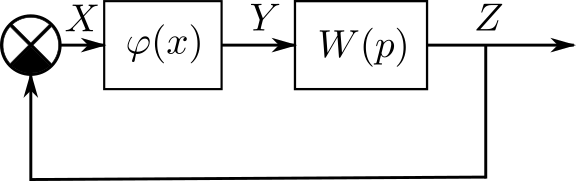
\includegraphics[width=.5\textwidth]{png/схема.png}
		\caption{Схема исследуемой НСАУ в виде модели Гаммерштейна}
		\label{scheme}
	\end{figure} 
	
	Линейная часть состоит из следующих звеньев, соединённых последовательно:
	\begin{align*}
		& W_1(p) = \frac{0,7}{p} \\
		& W_2(p) = \frac{1}{1+15p} \\
		& W_3(p) = \frac{1 + 2p}{1 + 20p}
	\end{align*}
	
	Нелинейный элемент (НЭ) задан характеристикой, которая представлена на рис. \ref{NE}.
	
	\begin{equation*}
		\varphi(x) = \begin{cases}
			1, &x\geq 1 \\
			2(x-\frac{1}{2}), &\frac{1}{2} \leq x \leq 1 \\
			0, &|x| \leq \frac{1}{2} \\
			2(x+\frac{1}{2}), &-1\leq x \leq -\frac{1}{2} \\
			-1, &x\leq -1
		\end{cases}
	\end{equation*}
	
	\begin{figure}[h]
		\centering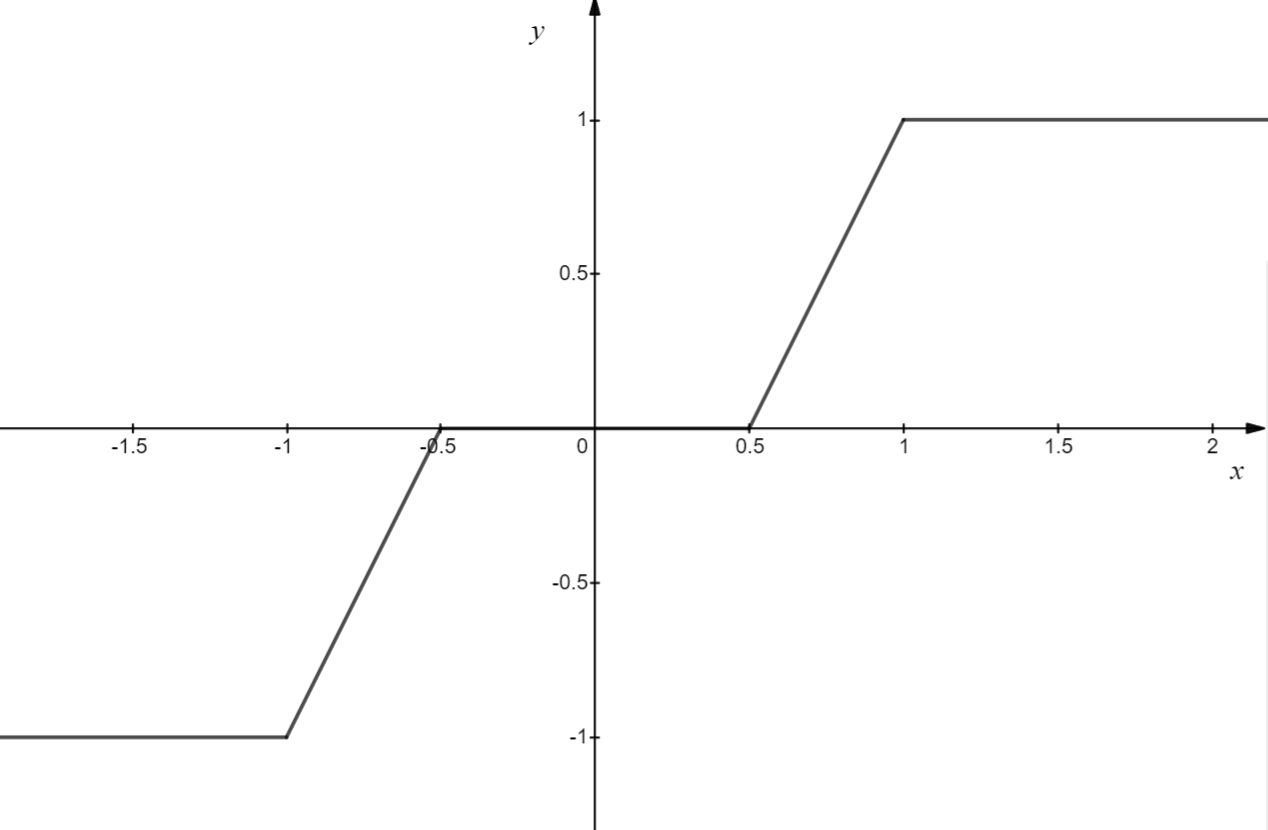
\includegraphics[width=.6\textwidth]{png/НЭ.png}
		\caption{Характеристика нелинейного элемента}
		\label{NE}
	\end{figure}
	
	Исследовать устойчивость отрезка равновесия и определить кривую граничных значений устойчивости, задаваемую парой коэффициент усиления $W_1(p)$ и постоянная времени $W_2(p)$.
	
	Для этого использовать три подхода: критерий Попова, метод Гольдфарба и непосредственное моделирование системы.
	
	\section{Подготовка к работе}
	
	Заметим, что нелинейная характеристика лежит в секторе $\dfrac{\varphi(x)}{x} \leq k_0 = 1$. Значит, прямая Попова будет проходить через точку $-\dfrac{1}{k_0} = -1$.
	
	Определим ожидаемый вид линейной части и отрицательной инверсной характеристики, которые используются в методе Гольдфарба.
	
	\begin{equation*}
		W_\text{лч} = \frac{0,7(1+2p)}{(1+15p)(1+20p)}
	\end{equation*}
	
	Эквивалентный комплексный коэффициент усиления (ЭККУ):
	\begin{equation*}
		W_\text{нэ}(A) = a(A) + jb(A)
	\end{equation*}
	
	Определим вид коэффициентов гармонической линеаризации:
	\begin{multline*}
		a(A) = \frac{1}{\pi A} \int_{-\pi}^\pi \varphi(A\sin{(\omega t)})\sin{(\omega t)}\dd{\omega t}\stackrel{\text{чёт}}{=} 
		\frac{2}{\pi A} \int_{0}^\pi \varphi(A\sin{(\omega t)})\sin{(\omega t)}\dd{\omega t} \stackrel{\text{симм}}{=} \\
		\stackrel{\text{симм}}{=} \frac{4}{\pi A} \int_{0}^{\frac{\pi}{2}} \varphi(A\sin{(\omega t)})\sin{(\omega t)}\dd{\omega t} \leq 
		\frac{4}{\pi A} \int_{0}^{\frac{\pi}{2}} \varphi(Ax)x\dd{x} = C_1 + \frac{C_2}{A}
	\end{multline*}
	
	Учитывая то, что коэффициент ряда Фурье $\alpha(A) = a(A)\cdot A$ является непрерывной, а значит, ещё и ограниченной функцией, можно отметить, что $a(0) = 0$ и $a(+\infty) =~0$. Это значит, что $a(A)$, как непрерывная функция, по теореме Ролля имеет по крайней мере один экстремум для некоторого значения $A$.
	
	Заметим, что $\int_{-\pi}^\pi \varphi(A\sin{(\omega t)})\sin{(\omega t)}\dd{\omega t}$ -- неубывающая функция аргумента $A$, которая перемножается с убывающей функцией $\dfrac{4}{\pi A}$. На этом основании можно утверждать, что экстремум $a(A)$ единственный.
		
	\begin{equation*}
		b(A) = \frac{1}{\pi A} \int_{-\pi}^\pi \varphi(A\sin{(\omega t)})\cos{(\omega t)}\dd{\omega t} \stackrel{\text{нечёт}}{=} 0
	\end{equation*}
	
	Итого построим качественно вид линейной части и инверсной характеристики $-z(A) = -\dfrac{1}{a(A)+jb(A)}$: рис. \ref{schematichno}.
	
	\begin{figure}[h]
		\centering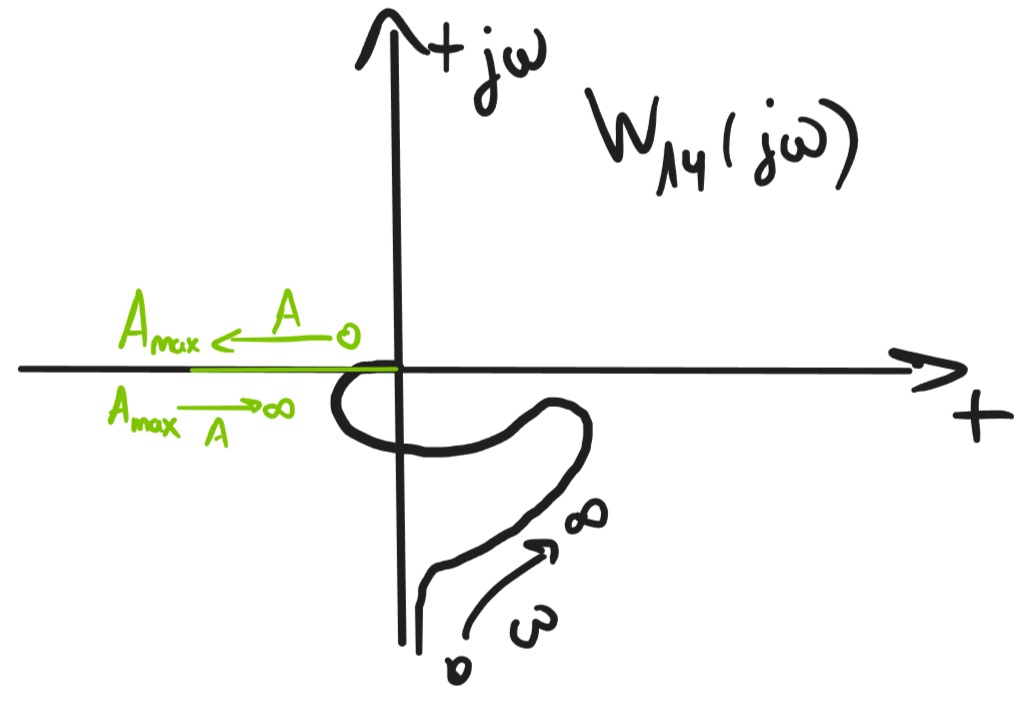
\includegraphics[width=.6\textwidth]{png/схематично.jpg}
		\caption{Качественный вид графического решения уравнения автоколебаний}
		\label{schematichno}
	\end{figure}
	
	\section{Выполнение работы}
	
	Исследуется устойчивость системы рис. \ref{scheme} с линейной частью:
	\begin{equation*}
		W_\text{лч} = \frac{k(1+2p)}{(1+Tp)(1+20p)}
	\end{equation*} 
	при различных значениях параметров $k,\,T$. Для этого будем строить графическую зависимость предельных значений устойчивости $T_\text{пр}(k_\text{пр})$.
	
	\subsection{Исследование устойчивости критерием Попова}
	
	Набор точек предельных значений в которых выполняется критерий В.~М.~Попова представлен на рис. \ref{popov1}. Также, на рис. \ref{popov1}-\ref{popov3} представлены виды модифицированной АФХ линейной части по отношению к прямой Попова для случаев предельного значения, не выполнения критерия и устойчивого положения равновесия по данному критерию.
	
	\begin{figure}
		\centering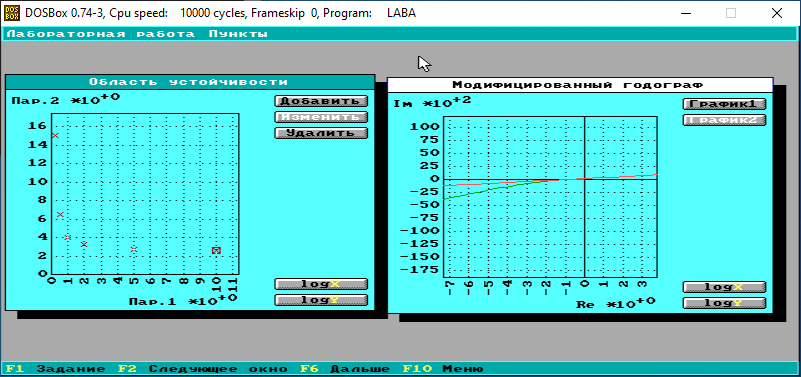
\includegraphics[width=.85\textwidth]{png/1.png}
		\caption{Предельное значение устойчивости по критерию}
		\label{popov1}
	\end{figure}
	
	\begin{figure}
		\centering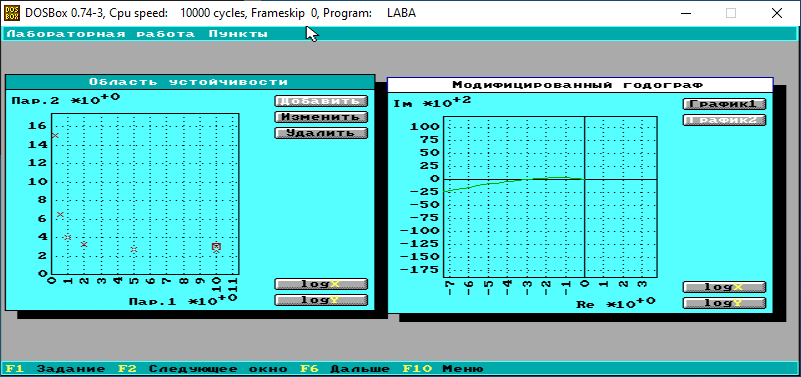
\includegraphics[width=.85\textwidth]{png/2.png}
		\caption{Значение, при котором критерий не выполняется}
		\label{popov2}
	\end{figure}
	
	\begin{figure}
		\centering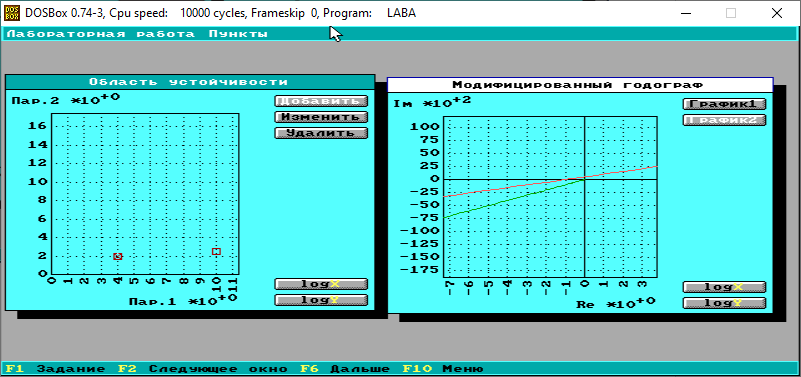
\includegraphics[width=.85\textwidth]{png/3.png}
		\caption{Устойчивое положение равновесия по критерию Попова}
		\label{popov3}
	\end{figure}
	
	\subsection{Метод гармонического баланса}
	
	Набор точек предельных значений по методу гармонического баланса представлен на рис. \ref{garm1}. Также, на рис. \ref{garm1}-\ref{garm3} представлены виды АФХ линейной части по отношению к отрицательной инверсной характеристике для случаев предельного значения наличия автоколебаний, наличия автоколебаний и отсутствия автоколебаний.
	
	\begin{figure}
		\centering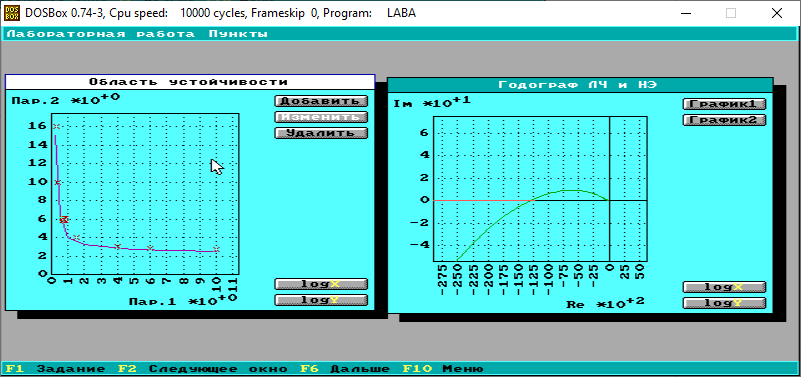
\includegraphics[width=.8\textwidth]{png/4.png}
		\caption{Предельное наличия автоколебаний}
		\label{garm1}
	\end{figure}
	
	\begin{figure}
		\centering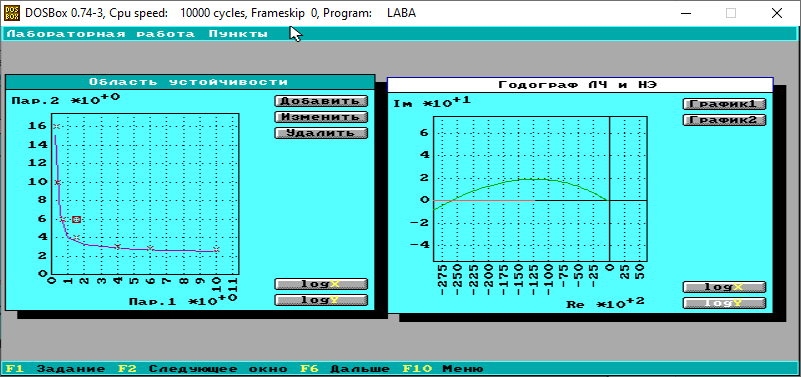
\includegraphics[width=.8\textwidth]{png/5.png}
		\caption{Значение, при котором присутствуют автоколебания}
		\label{garm2}
	\end{figure}
	
	\begin{figure}
		\centering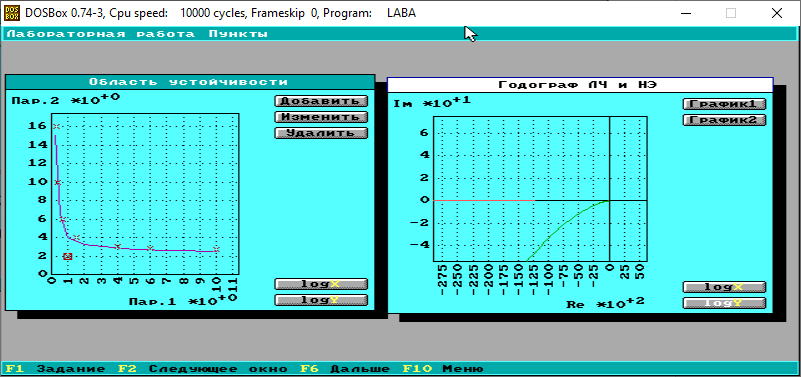
\includegraphics[width=.8\textwidth]{png/6.png}
		\caption{Значение, при котором отсутствуют автоколебания}
		\label{garm3}
	\end{figure}
	
	\subsection{Моделирование процессов системы}
	
	Набор точек предельных значений по непосредственному моделированию системы представлен на рис. \ref{mod1}. Также, на рис. \ref{mod1}-\ref{mod3} переходные процессы системы для случаев незатухающего переходного процесса, неустойчивого процесса и затухающего процесса.
	
	\begin{figure}
		\centering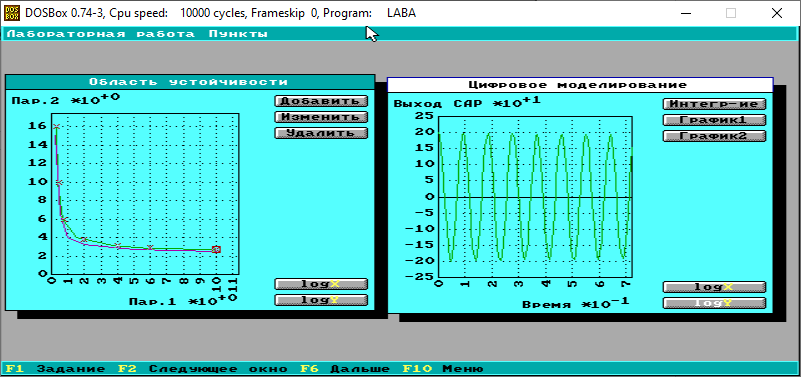
\includegraphics[width=.8\textwidth]{png/7.png}
		\caption{Незатухающий переходной процесс}
		\label{mod1}
	\end{figure}
	
	\begin{figure}
		\centering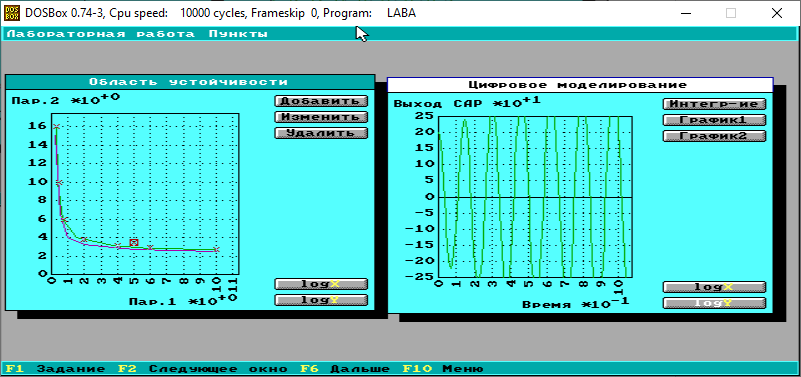
\includegraphics[width=.8\textwidth]{png/8.png}
		\caption{Неустойчивый переходной процесс}
		\label{mod2}
	\end{figure}
	
	\begin{figure}
		\centering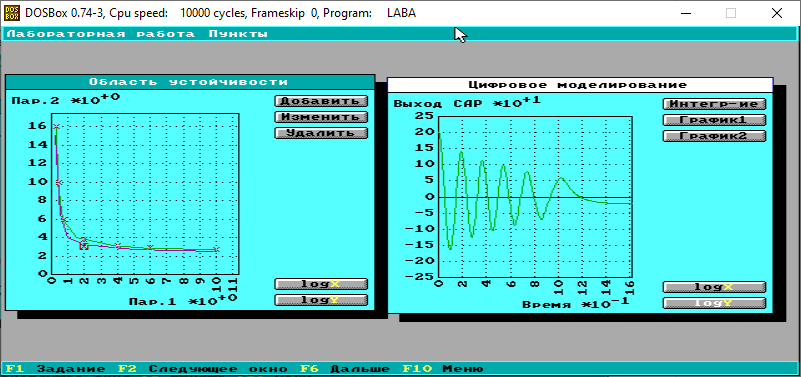
\includegraphics[width=.8\textwidth]{png/9.png}
		\caption{Затухающий переходной процесс}
		\label{mod3}
	\end{figure}
	
	\subsection{Подведение итогов}
	
	Полученные граничные кривые устойчивости представлены на рис. \ref{itog}. Фиолетовым отмечен результат по критерию Попова. Зелёным по методу гармонического баланса. Красным результат, полученный непосредственным моделированием.
	
	\begin{figure}[h]
		\centering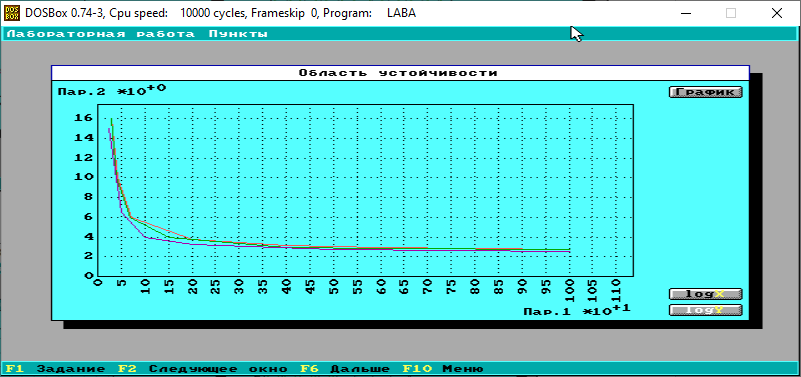
\includegraphics[width=.9\textwidth]{png/Итог.png}
		\caption{Полученные кривые $T_\text{пр}(k_\text{пр})$}
		\label{itog}
	\end{figure}
	
	Эталонным результатом можно считать кривую, полученную моделированием, поскольку в таком подходе нет ограничений методических или случаев, когда подход не даёт ответа на вопрос об устойчивости. Единственная ошибка вносится погрешностью численного моделирования, но она может быть ограничена заданной точностью расчёта.
	
	Как видим по характеру и значениям все три кривые оказались очень похожими. Кривая по критерию Попова оказалась наиболее ограничивающей к области, в которой положение равновесия системы считается устойчивым. Это связано с тем, что критерий является достаточным, и в случае его невыполнения положение равновесия может так же оказаться устойчивым.
	
	Результат, полученный по методу Гольдфарба оказался очень близок к эталонному. Это связано с тем, что предположение метода о фильтре было приближённо выполнено, из-за чего метод дал близкие к истине результаты.
	
	\section{Выводы}
	
	В данной работе была исследована устойчивость положения равновесия НСАУ относительно двух параметров из её линейной части.
	
	Такое исследование было проведено с помощью трёх подходов: критерия Попова, метода гармонического баланса и компьютерного моделирования.
	
	Все три подхода дали близкие результаты: критерий Попова выделил меньшую область устойчивости положения равновесия, но по характеру граничных значений был получен тот же результат.

\end{document}
